\documentclass{article}
\usepackage{natbib}
\usepackage[labelfont=bf]{caption}
\usepackage{subcaption}
\usepackage{graphicx}
\usepackage{float}
\bibliographystyle{apalike}
\usepackage{lineno}
\linenumbers

\usepackage{geometry}
\geometry{letterpaper}
\geometry{margin=1in}

\usepackage{setspace}
\doublespacing
\captionsetup[figure]{font={stretch=2}}

\usepackage{authblk}
\usepackage{xcolor}

\newcommand{\matr}[1]{\mathbf{#1}}

\title{Improving Accuracy of Simulated Flows in Steeply Dipping Layers Using Vertically Staggered Grids with the XT3D Multi-Point Flux Approximation in MODFLOW 6}
\author{
	Alden M. Provost, U.S. Geological Survey, Integrated Modeling and Prediction Division, U.S. Geological Survey, 12201 Sunrise Valley Dr, Reston, VA, USA  \\
	\and 
	Kerry Bardot, School of Earth Sciences, University of Western Australia, Perth, Australia \\
	\and 
	Christian D. Langevin, U.S. Geological Survey, Integrated Modeling and Prediction Division, 2280 Woodale Drive, Mounds View, MN, USA \\
	\and 
	James L. McCallum, School of Earth Sciences, University of Western Australia, Perth, Australia \\
	}


\date{\today}

\begin{document}

\maketitle

\textbf{Conflict of interest:} None.

\textbf{Key words:} groundwater flow simulation, dipping model layers, vertically staggered grid, multi-point flux approximation

\textbf{Article impact statement:} {\color{red} AMP: Need impact statement}

\begin{abstract}
\noindent {\color{red} AMP: compose Abstract near the end}
\end{abstract}

\section{Introduction}

In the MODFLOW family of hydrologic simulation codes, a groundwater model domain is discretized into a grid of hydraulically connected model cells. Versions of MODFLOW up to and including MODFLOW-2005 \citep{modflow2005} offered only structured grids composed of rows, columns, and layers of cells. Cells were conceptualized as having horizontal top and bottom surfaces, which allowed each cell to be ``simulated as if it were rectangular so that flow may be approximated by the standard finite-difference equation" \citep{modflow84}. In MODFLOW-USG \citep{modflowusg} and MODFLOW 6 \citep{modflow6gwf}, which offer unstructured grids and use the control-volume finite-difference method to formulate the discrete balance equations, cells continue to have horizontal tops and bottoms, which simplifies the definition and calculation of water-table elevations, cell saturations, and hydraulic conductances between cells.

A traditional approach to representing an aquifer system with dipping hydrogeologic layers in MODFLOW is to map the hydrologic properties onto a rectilinear grid \citep{modflow84}. Another approach available in all versions of MODFLOW is to allow the top and bottom elevations of cells in the same layer of the grid to vary spatially. Following \cite{bardot2022}, in this work we call this type of grid ``vertically offset." The vertical offsets between ``horizontally" adjacent cells allows model layers to ``deform'" with the hydrostratigraphy to ``minimize the number of model layers required to simulate an aquifer system" \citep{modflow84} relative to a rectilinear grid with horizontal layers. In both approaches, the model grid follows the boundaries of dipping layers approximately, in what \cite{bardot2022} call a ``staircase" fashion.

All versions of MODFLOW prior to MODFLOW 6 used a two-point, ``conductance-based" flow formulation in which the flow between two adjacent cells is proportional to the difference between the heads calculated in those two cells. The conductance-based flow formulation is most accurate when the grid satisfies the ``control-volume finite-difference (CVFD) requirement" that the straight-line connection between two cell centers must intersect the midpoint of the cell interface at a right angle \citep{narasimhan1976integrated}. However, vertically offset grids violate the CVFD requirement because cell interfaces are vertical but cell connections are not strictly horizontal. For this reason, the MODFLOW 6 documentation \citep{modflow6gwf} warns that "[s]teeply dipping layers generally should not be represented" using vertical offsets. \cite{anderson2015applied} recommend a $10^{\circ}$ dip as a practical upper limit for using vertical offsets.

To improve the accuracy of flow simulations on unstructured grids, and to allow accurate simulation of arbitrarily oriented two- or three-dimensional anisotropy, the optional XT3D flow formulation \citep{modflow6xt3d} was introduced in MODFLOW 6. By performing flow calculations using Darcy's Law in its tensorial form based on a multi-point approximation of the head gradient vector, XT3D accounts for both arbitrarily oriented anisotropy and geometric irregularity of the grid. In theory, XT3D should be able to compensate for the geometic irregularity introduced by vertical offsets between adjacent cells in the same model layer.

\cite{bardot2022} evaluated the effects of grid design and XT3D on the ability of MODFLOW 6 to accurately simulate flow through sedimentary structures by modeling an idealized, two-dimensional permeable channel or hydrogeologic layer embedded in a nearly impermeable surrounding medium, or ``domain." In their plan-view benchmark, the channel lay within the horizontal plane as was angled counterclockwise relative to the southern boundary of the model domain (by $30^{\circ}$ in most cases). Constant-head boundary conditions at the ends of the channel were set to induce uniform flow along the channel in the corresponding analytical solution. The channel and surrounding domain were discretized using either a rectilinear grid, which satisfies the CVFD requirement, or a ``flexible triangular" grid that is unstructured with triangular cells and does not satisfy the CVFD requirement. They found that the standard, conductance-based flow formulation gave accurate results on the rectilinear grid but was subject to significant error on the unstructured grid, whereas the XT3D flow formulation gave accurate results on both grids, as expected. However, in the transect (cross-sectional) version of their benchmark, which used a vertically offset grid to discretize the nearly impermeable domain and a permeable channel (hydrogeologic layer) inclined by $30^{\circ}$ from the horizontal, similarly poor results were observed with and without XT3D. Given the ability of XT3D to compensate for violations of the CVFD requirement, it appeared likely that another aspect of the problem formulation or the inner workings of MODFLOW 6 was responsible for the unexpected results. As noted by \cite{bardot2022}, a preliminary analysis by two authors of the present work (Provost and Langevin) suggested that the cell connectivity offered by a vertically offset grid was inadequate for allowing an accurate flow solution. 

"Vertically staggered" grid connections were introduced in MODFLOW-USG \citep{modflowusg} and included for the fully unstructured (DISU) grid type in MODFLOW 6 \citep{modflow6gwf} primarily as a means to vertically subdiscretize portions of a grid that are conceptualized as being layered. A grid that includes vertically staggered connections, which in this work we call a ``vertically staggered grid," some cells have nominally ``horizontal" connections with more than one cell across a given cell face. Vertically staggered DISU grids allow more flexibility in assigning grid connectivity than do the more commonly used DIS and DISV grid types \citep{modflow6gwf} in MODFLOW 6. To our knowledge, the implications of limited grid connectivity for the accuracy of simulated flows in models with steeply dipping layers, and the potential for using vertically staggered grids to overcome this limitation, have not been previously appreciated or investigated.

In the remainder of this paper we first present a theoretical justification for the hypothesis that inadequate grid connectivity is primarily responsible for the inaccurate simulation of flows in the steeply dipping layer benchmark on a vertically offset grid. Based on that theory, we propose a method for improving the accuracy of the flow solution using XT3D together with a vertically staggered grid, and we evaluate the effectiveness of that approach in a set of benchmark problems similar to those of \cite{bardot2022}. Finally, we discuss the potential implications of our findings for practical groundwater models that include high permeability contrasts and steeply dipping layers.

{\color{red} AMP: terminology -- ``channel" vs ``hydrogeologic layer"? ``hydrogelogic layer" vs ``model layer"?}

{\color{red} AMP: Random thoughts
\begin{itemize}
	\item Vertical offset happens even on a completely rectilinear grid if the water table elevation varies in horizontally adjacent cells. Doesn't seem like the same kind of issue, but think on it. But not now, I think.
	\item Could mention the crossflow case briefly in this paper, like \cite{bardot2022} mentioned this work as something we were looking into at the time.
	\item Could try making the channel less permeable than the domain; semi-confining unit. Thinking not now.
	\item Difference between truly single-layer model of channel vs embedded single-layer channel -- no vertical connections vs vertical connections that are no-flux. Effect on specific discharge calculations? Relevance of the specific-discharge "patch"? But beyond that, Kerry suggested that it's important to investigate and describe the embedded single-layer case, as it's a common use case, and she did some runs -- email of 2022-09-29.  With or without xt3d, the results were not good, and I'm not sure it's possible to get good results, since there's no way to introduce cross-connections within a single-layer channel.  Would be good to explain this in the paper.  (She also tried a vertical gradient for the embedded single-layer case, also with poor results, though this might also have something to do with the cross-flow, "heterogeneity correction" issue.)
\end{itemize}
}

\section{Theoretical Background}

\begin{figure}
	\begin{center}
%	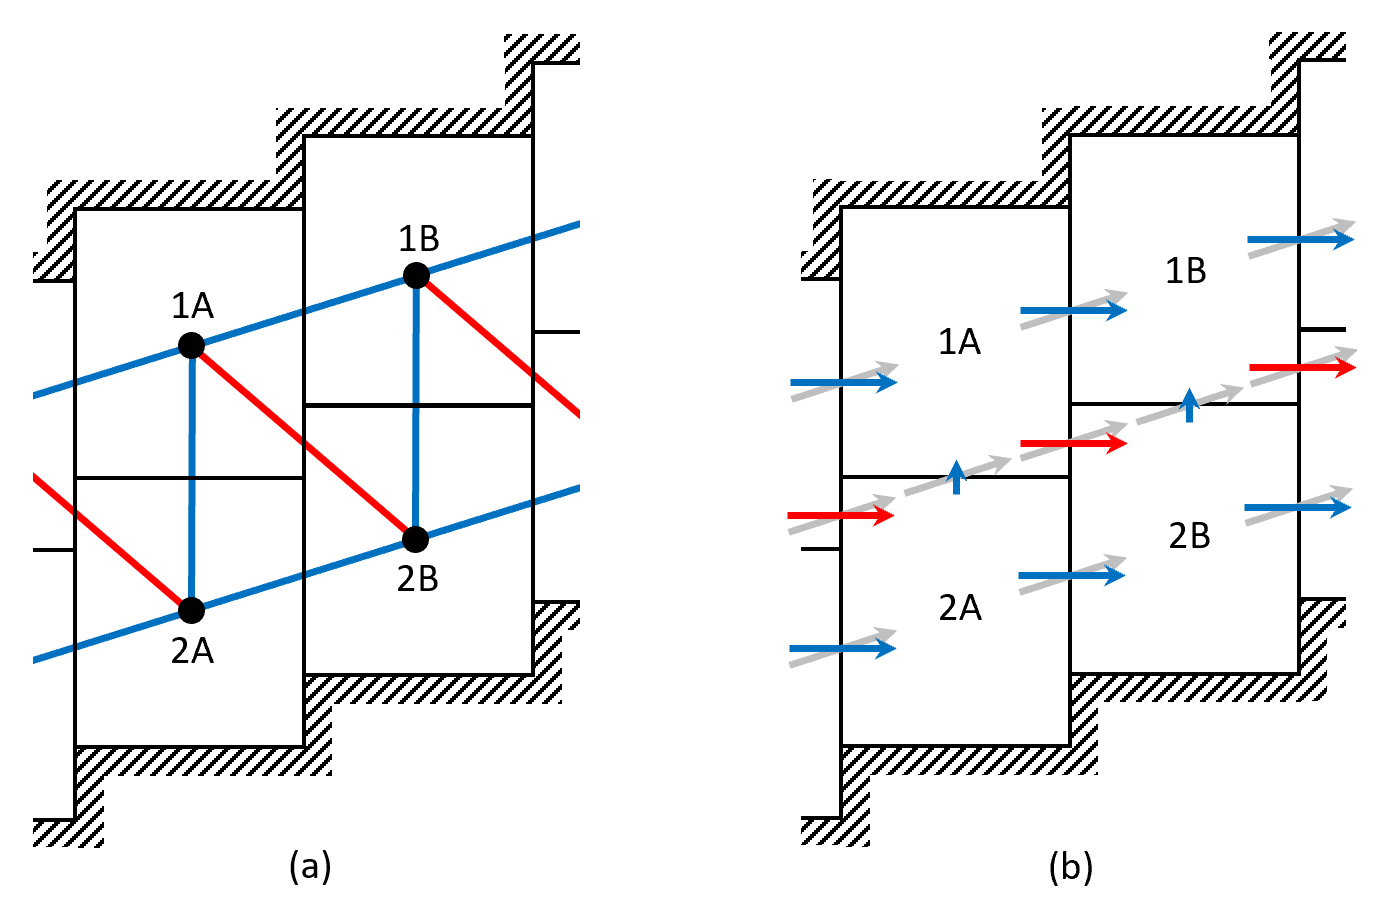
\includegraphics[scale=0.8]{../figures/schem_conn_area_flux.png}
	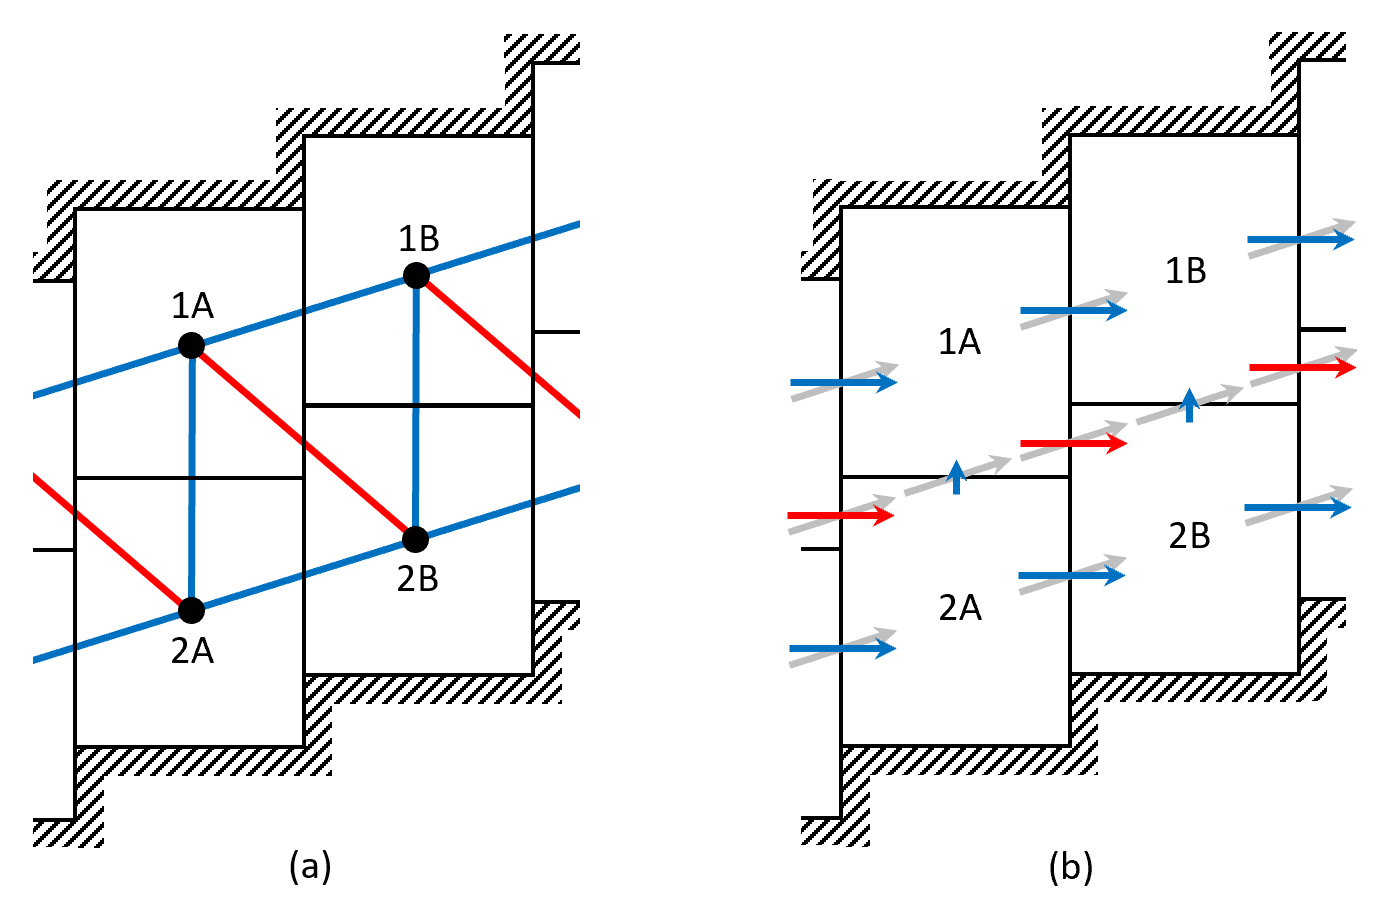
\includegraphics[scale=0.6]{../figures/schem_conn_area_flux.png}
	\caption{Schematics showing (a) grid connectivity and (b) cell interface fluxes in a two-layer model of a dipping channel. Hatching denotes impermeable boundaries along the top and bottom of the channel. In (a), black circles represent cell centers. Blue lines represent hydraulic connections between cells in a vertically offset grid. Red lines represent additional connections that result in a vertically staggered grid. In (b), gray arrows represent the uniform groundwater flux the model is attempting to simulate. Blue arrows represent components of the uniform groundwater flux normal to the horizontal and vertical cell-cell interfaces in the vertically offset grid. Red arrows represent components of the uniform groundwater flux normal to the additional vertical cell-cell interfaces introduced in the vertically staggered grid.}
	\label{fig:schem-conn-area-flux}
	\end{center}
\end{figure}

Figure \ref{fig:schem-conn-area-flux}a shows a group of four cells in a two-layer, cross-sectional MODFLOW 6 model of fully saturated flow through a permeable channel (aquifer) with impermeable top and bottom boundaries. The cells have horizontal tops and bottoms and can therefore follow the dip of the channel only on average, in what \cite{bardot2022} refer to as ``staircase" fashion. If the grid is represented using a layered grid type (DIS or DISV) in MODFLOW 6, a cell is hydraulically connected to each cell in the same layer with which it has an overlapping face and with each cell in an adjacent layer with which it shares a horizontal face, as indicated by the blue lines that connect cell centers in figure \ref{fig:schem-conn-area-flux}a. Following \cite{bardot2022}, in this work we call this type of grid ``vertically offset" because the tops and bottoms of adjacent cells in the same layer are not necessarily aligned. Note that cells that have overlapping vertical faces but are in different layers (e.g., cells 1A and 2B) do not have a direct hydraulic connection in a vertically offset grid. The addition of such connections between cells in different layers, as indicated by the red lines that connect cell centers in figure \ref{fig:schem-conn-area-flux}a, results in a ``vertically staggered" grid. The ability to handle vertically staggered grids was first introduced to MODFLOW by \cite{modflowusg} in MODFLOW-USG, and the term ``vertically staggered" was first used by \cite{modflow6gwf} in the context of MODFLOW 6. The term describes a grid in which which a cell can have nominally ``horizontal" connections with with multiple cells across the same cell face. In this work, ``vertically offset" and ``vertically staggered" are used to distinguish grids that lack nominally ``horizontal" connections between cells in adjacent layers (red lines in figure \ref{fig:schem-conn-area-flux}a) from those that include such connections, respectively.  In the vertically offset grid in \ref{fig:schem-conn-area-flux}a (blue connections only), the interfacial area across which flow occurs between adjacent cells in the same layer is based on the vertical cell thickness (the entire thickness of the channel). In the vertically staggered grid (blue and red connections), the interfacial area for nominally ``horizontal" flow between adjacent cells is based on the area over which the two cell faces overlap. Thus, while the total area for nominally ``horizontal" flow across a cell face is the same as for a vertically offset grid, that total area is divided between an adjacent cell in the same layer (blue connection) and an adjacent cell in the adjacent layer (red connection). In MODFLOW 6, vertically offset grids can be represented using the structured (DIS), vertex-based (DISV), or fully unstructured (DISU) grid type, whereas vertically staggered grids can be represented only using the DISU grid type.

In MODFLOW 6, the default method for representing the flow between two hydraulically connected model cells is the ``conductance-based flow formulation" \citep{modflow6gwf}. In this formulation, which is based on the commonly used two-point flux approximation {\color{red} *** ref? ***}, the flow is proportional to the difference in the hydraulic heads computed at the two cell centers and a hydraulic conductance based on an effective hydraulic conductivity for the connection between the cells. On strictly rectilinear grids, such as structured MODFLOW grids with no vertical offset between cells in the same layer, with hydraulic conductivity that is isotropic or has anisotropy aligned with the three mutually perpendicular grid directions, the conductance-based formulation is second-order accurate \citep{dehotin2010modeling, modflow6gwf}. This is because strictly rectilinear grids satisfy the ``control-volume finite-difference (CVFD) requirement" that the straight-line connection between two cell centers must intersect the midpoint of the cell interface at a right angle \citep{narasimhan1976integrated}. Vertically offset grids, however, violate the CFVD requirement because nominally ``horizontal" connections between cell centers in the same layer are not strictly horizontal and therefore not perpendicular to the vertical cell interfaces they intersect. For example, in figure \ref{fig:schem-conn-area-flux}a, the connection between cells 1A and 1B is not perpendicular to the cell interface, which compromises the accuracy of the conductance-based formulation.

The conductance-based formulation was the only flow formulation available in versions of MODFLOW prior to MODFLOW 6. As mentioned earlier, the limitations of the conductance-based formulation on vertically offset grids were well recognized. However, the ability to use unstructured grids in MODFLOW-USG and MODFLOW 6 introduced the potential to violate the CVFD requirement, and thereby render the conductance-based formulation less accurate, even in the absence of vertical offsets. To improve accuracy on unstructured grids, and to allow accurate simulation of arbitrarily oriented two- or three-dimensional anisotropy, the optional XT3D flow formulation \citep{modflow6xt3d} was introduced in MODFLOW 6. XT3D formulates the flow between two cells by interpolating head values from the two cells and their neighboring cells to construct an estimate of the full, two- or three-dimensional head-gradient vector on each side of the cell interface; applying the cell conductivity tensors to obtain an estimate of the groundwater flux vector on each side of the interface; and reconciling the two flux estimates to ensure continuity of flow across the interface. By performing flow calculations using Darcy's Law in its tensorial form, based on a ``multi-point" approximation of the head gradient, XT3D accounts for both arbitrarily oriented anisotropy and geometric irregularity of the grid.

The dipping-channel benchmark problem of \cite{bardot2022} used a vertically offset grid, which is the type of grid used most often in MODFLOW models. Test simulations using the conductance-based flow formulation for a steeply dipping channel (hydrogeologic layer) embedded in a domain that is six orders of magnitude less hydraulically conductive yielded significant errors in the simulated flows. The simulated groundwater flux in the middle of the channel was not along the $30^{\circ}$ incline of the channel, but nearly horizontal ($0.03^{\circ}$ incline), and its magnitude was overestimated by 15\%. Significant errors in the simulated flows were expected in this case, given that the conductance-based flow formulation does not rigorously account for violations of the CVFD requirement that the cell-cell connection be perpedicular to the cell-cell interface, and that it takes the connection length to be the horizontal distance between cell centers.  Given the ability of XT3D to account rigorously for grid connections that are not perpendicular to cell interfaces, and for the increase in connection length due to the slope of the connection, rerunning the simulation with XT3D activated could have been expected to improve the flow solution substantially. However, \cite{bardot2022} observed similarly poor results with XT3D: the flux was still nearly horizontal ($0.01^{\circ}$ incline), and its magnitude was overestimated by 12\%. Based on a preliminary analysis by two authors of the present work (Provost and Langevin), \cite{bardot2022} hypothesized that the unexpectedly large error in the flow solution with XT3D was related to indequate grid connectivity was at the root of the problem.

The role of grid connectivity in enabling accurate simulation of flow along a dipping channel can be understood by considering figure \ref{fig:schem-conn-area-flux}b, in which components of the groundwater flux (specific discharge) vector representative of steady, uniform flow along the channel are superimposed on each cell interface. Gray vectors represent the uniform flux oriented along the channel, which the model is attempting to simulate. Blue vectors represent the flux components normal to cell interfaces that correspond to blue connections in figure \ref{fig:schem-conn-area-flux}a, which are common to both the vertically offset and vertically staggered grids. Red vectors represent the flux components normal to cell interfaces that correspond to red connections in figure \ref{fig:schem-conn-area-flux}a, which are lacking in the vertically offset grid.

The blue vectors in figure \ref{fig:schem-conn-area-flux}b show that to simulate steady, uniform flow along the dipping channel, cells must exchange water not only ``horizontally" with neighboring cells in the same layer, but also vertically with cells in the adjacent layer. Specifically, there must be flow from cells in the bottom layer to cells in the top layer, which corresponds to the vertical component of the groundwater flux. Note, however, that the blue vectors alone are incompatible with steady, uniform flow along the channel because the exchange of water between the two model layers is in one direction only: upward. Such a steady-state flow configuration would imply continuous depletion of flow within the bottom layer and accumulation of flow within the top layer as one moves along the channel in the direction of flow. Thus, steady, uniform flow along the channel cannot be simulated accurately without some mechanism for returning flow from the top layer to the bottom layer. The vertically staggered grid provides such a mechanism by offering additional connections between cells in adjacent layers. Vertical flows from the bottom layer to the top layer, represented by vertical blue vectors in figure \ref{fig:schem-conn-area-flux}b, can be returned to the bottom layer by nominally ``horizontal" flows, represented by red vectors in figure \ref{fig:schem-conn-area-flux}b. Although this concept has been illustrated using a two-layer model for simplicity, the same reasoning applies given any number of layers.

Once the appropriate connectivity is established using a vertically staggered grid, it is the role of the flow formulation to account properly for the geometry of the grid, a task for which XT3D was specifically designed. However, XT3D alone cannot compensate for grid connectivity that does not provide adequate pathways for flow. This explains why using XT3D did not improve the simulation results substantially on a vertically offset grid in the benchmark tests of \cite{bardot2022}.  In the middle section of the channel, away from the end boundary conditions, the flow solution approached steady, uniform flow the only way that it could given the limited connectivity of the vertically offset grid: by suppressing vertical flows between layers, thereby rendering the overall flow approximately horizontal.

The arguments presented in this section suggest that, in addition to the use of XT3D, the enhanced connectivity provided by a vertically staggered grid can be important for obtaining an accurate flow solution in MODFLOW 6 simulations that involve steeply dipping layers. The next section presents results of simulations designed to test this hypothesis.

\section{Description of Test Problems}

The test problems are patterned after the cross-sectional (transect) benchmarks of \cite{bardot2022}. They attempt simulate uniform flow in a permeable channel embedded in a less permeable surrounding ``domain." The channel is of uniform width and hydraulic conductivity and is inclined relative to the horizontal.

To simulate flow along a channel inclined at angle $\theta$, heads are specified at the centers of cells along the perimeter of the model {\color{red} (AMP: this assumes we're using the transect\_benchmark version of the model, which includes the "domain," for all of our final runs)} using an analytical solution that corresponds to a unit head gradient inclined at angle $\theta$ \citep{bardot2022}:

\begin{equation}
\label{eqn:head_analyt_along}
h = - x \cos \theta - z \sin \theta.
\end{equation}

\noindent where $h$ is head in meters and $x$ and $z$ are the horizontal and vertical model coordinates, respectively, in meters. The hydraulic conductivity of the channel is set to 1 m/d (meter per day) so that the analytical flow solution is a groundwater flux of 1 m/d either along or across the channel. The conductivity of the domain surrounding the channel varies according to the scenario being investigated. In the homogeneous limit, the conductivity of the domain is set equal to that of the channel. In the highly heterogeneous limit, the conductivity of the domain is set much lower than that of the channel to effectively isolate the channel hydraulically.

Simulations are performed using variations on two test problems that differ in their method of discretization. The first test problem uses the traditional approach of representing the inclined channel using a vertically offset grid of the MODFLOW 6 DIS (structured) type. {\color{red} (AMP: present results for the DIS grid, or for the equivalent of the DIS grid after conversion to DISU?)} This problem confirms the findings of \cite{bardot2022} and illustrates the limitations of the vertically offset grid approach. The second test problem is similar to the first but uses a vertically staggered grid of MODFLOW 6 DISU (unstructured) type. The second problem is designed to evaluate the effectiveness of cross-connections between layers (illustrated in figure \ref{fig:schem-conn-area-flux}c) in improving the accuracy of the flow solution, both with and without XT3D. Variations on both test problems are described in the ``Results and Discussion" section.

Jupyter notebooks for both test problems are available in the Supporting Information that accompanies this paper. The notebooks leverage the capabilities of FloPy \citep{bakker2016scripting} to assist in setting up input for and processing results from the MODFLOW 6 simulations. The second test problem is formulated by starting with a DIS grid, converting it to an equivalent DISU grid, and adding cross-connections. A Python script for converting and modifying the grid is included.

\section{Results and Discussion}

{\color{red} AMP: Note that there's a temporary ``preliminary results" section at the end of the manuscript.}

{\color{red} AMP: Obviously need to substitute in our "real" results with "real" discussion and captions here.}

{\color{red} AMP: Based on the release notes, looks like the specific-discharge ``patch" went into v6.3.0. Mention it? Note that here is still the issue of coordinate dependence.}

{\color{red} AMP: Results without the domain are presented first to "cleanly" illustrate the main problem and its solution. Results with the domain are then presented to give more of an indication of how things might work in practice. Kerry has suggested that perhaps the cases with the domain are sufficient -- let's consider.}

{\color{red} AMP: Unless stated otherwise, the domain is 6 orders of magnitude less conductive than the channel, as in \cite{bardot2022}.}

{\color{red} AMP: Add and discuss results for how the flow error varies with discretization.  See plots in Kerry's emails of 2022-10-06 and 2022-12-14.}

{\color{red} AMP: Add and discuss results for how the flow error varies with dip angle. See plots in Kerry's email of 2022-12-14. "Spike" at 45 degrees due to "disconnection?"}

{\color{red} AMP: Add and discuss results for how the flow error varies with K contrast between channel and domain (heterogeneity).  See plots in Kerry's email of 2022-12-14.}

{\color{red} AMP: For consistency, should choose one notebook or the other for all runs.}

\subsection{Test Problem 1: Vertically Offset Discretization}

\begin{figure}[H]
\centering
\begin{subfigure}{0.4\textwidth}
	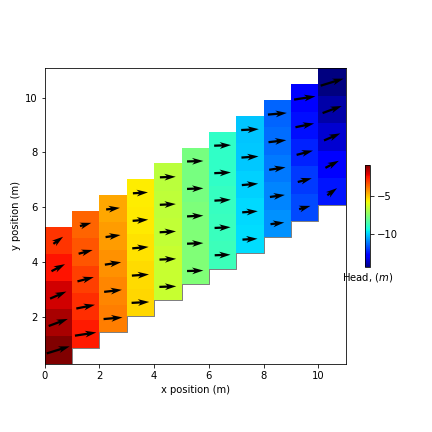
\includegraphics[width=\textwidth]{../figures/disu-af-vo-s-head.png}
	\caption{vertically offset grid, standard conductance-based formulation}
	\label{fig:disu-s-nocc-head}
\end{subfigure}
\hfill
\begin{subfigure}{0.4\textwidth}
	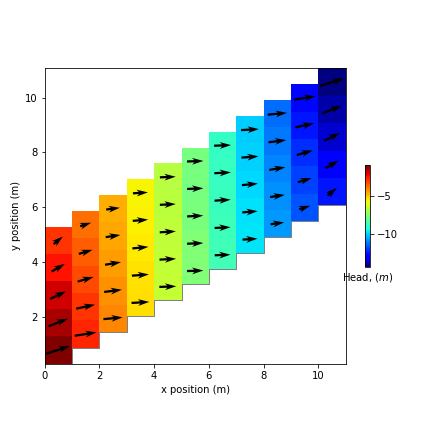
\includegraphics[width=\textwidth]{../figures/disu-af-vo-x-head.png}
	\caption{vertically offset grid, XT3D}
	\label{fig:disu-x-nocc-head}
\end{subfigure}
\caption{Specific discharge and head for a vertically offset grid. As Kerry and Jim found previously, the news is all bad; the flow tends to go horizontal, and XT3D doesn't really help. (preliminary result from disu\_approach model, 5x11 grid without cross-connections, $30^{\circ}$ incline, set up for flow along the channel; scenarios disu-af-vo-s and disu-af-vo-x)}
\label{fig:figures}
\end{figure}

\subsection{Test Problem 2: Vertically Staggered Discretization}

\begin{figure}[H]
\centering
\begin{subfigure}{0.4\textwidth}
	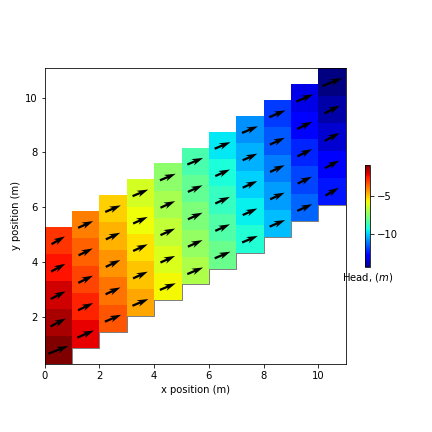
\includegraphics[width=\textwidth]{../figures/disu-af-vs-s-head.png}
	\caption{vertically staggered grid, standard conductance-based formulation}
	\label{fig:disu-s-cc-head}
\end{subfigure}
\hfill
\begin{subfigure}{0.4\textwidth}
	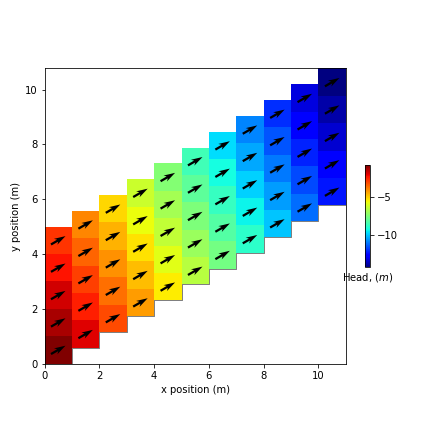
\includegraphics[width=\textwidth]{../figures/disu-af-vs-x-head.png}
	\caption{vertically staggered grid, XT3D}
	\label{fig:disu-x-cc-head}
\end{subfigure}
\caption{Specific discharge and head for a vertically staggered grid with cross-connections. The news is much better; the standard formulation is much improved, and XT3D nails it. (preliminary result from disu\_approach model, 5x11 grid with cross-connections, $30^{\circ}$ incline, set up for flow along the channel; scenarios disu-af-vs-s and disu-af-vs-x)  {\color{red} AMP: If keeping, combine with fig 3.}}
\label{fig:figures}
\end{figure}

\subsection{Test Problem 3: Vertically Offset Discretization with Domain}

\begin{figure}[H]
\centering
\begin{subfigure}{0.4\textwidth}
	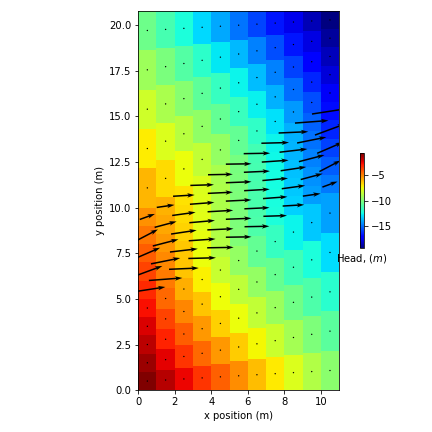
\includegraphics[width=\textwidth]{../figures/disu-d-af-vo-s-head.png}
	\caption{vertically offset grid, standard conductance-based formulation}
	\label{fig:disu-s-nocc-head}
\end{subfigure}
\hfill
\begin{subfigure}{0.4\textwidth}
	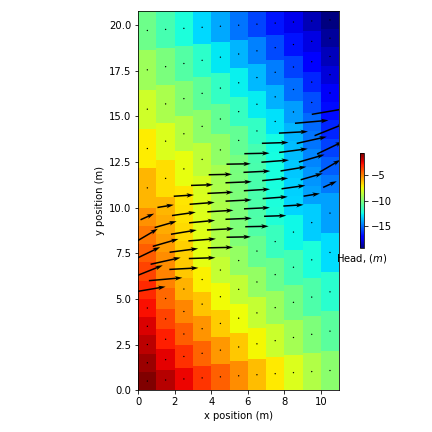
\includegraphics[width=\textwidth]{../figures/disu-d-af-vo-x-head.png}
	\caption{vertically offset grid, XT3D}
	\label{fig:disu-x-nocc-head}
\end{subfigure}
\caption{Specific discharge and head for a vertically offset grid with the domain. Results are similar to those without the domain and consistent with what Kerry and Jim found previously; the flow tends to go horizontal, and XT3D doesn't really help. (preliminary result from disu\_approach model, 5x11 channel with 5x11 subdomains above and below, without cross-connections, $30^{\circ}$ incline, set up for flow along the channel; scenarios disu-d-af-vo-s and disu-d-af-vo-x)}
\label{fig:figures}
\end{figure}

\subsection{Test Problem 4: Vertically Staggered Discretization with Domain}

\begin{figure}[H]
\centering
\begin{subfigure}{0.4\textwidth}
	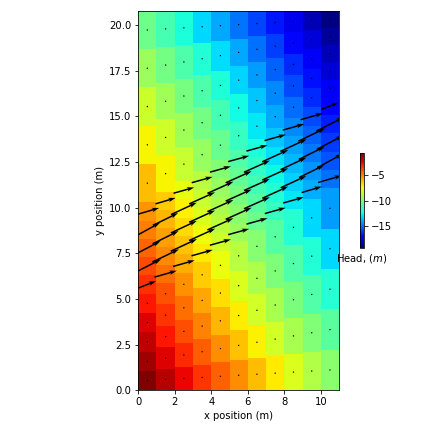
\includegraphics[width=\textwidth]{../figures/disu-d-af-vs-s-head.png}
	\caption{vertically staggered grid, standard conductance-based formulation}
	\label{fig:disu-s-cc-head}
\end{subfigure}
\hfill
\begin{subfigure}{0.4\textwidth}
	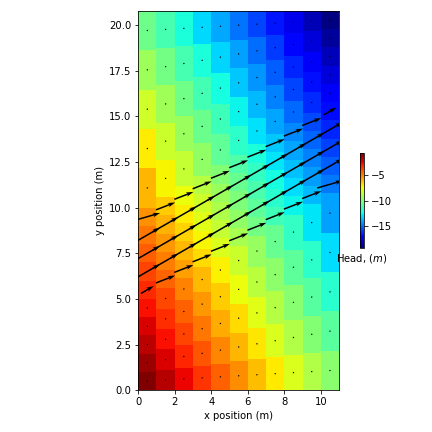
\includegraphics[width=\textwidth]{../figures/disu-d-af-vs-x-head.png}
	\caption{vertically staggered grid, XT3D}
	\label{fig:disu-x-cc-head}
\end{subfigure}
\caption{Specific discharge and head for a vertically staggered grid with the domain and with cross-connections. The standard formulation isn't horrible, and XT3D does very well except at the channel boundary, where there's presumably a "staircase" effect. (preliminary result from disu\_approach model, 5x11 channel with 5x11 subdomains above and below, with cross-connections, $30^{\circ}$ incline, set up for flow along the channel; scenarios disu-d-af-vs-s and disu-d-af-vs-x) {\color{red} AMP: Combine with fig 4.} {\color{red} AMP: Explain boundary anomalies.}}
\label{fig:figures}
\end{figure}

\section{Conclusions}

{\color{red} AMP: Need conclusions.}

{\color{red} AMP: The concepts in this paper have been easiest to discuss in terms of grid layers, but they're not limited to layered grids.}

\section{Acknowledgments}
{\color{red} AMP: Need acknowledgments.}

\section{Supporting Information}

\section{Appendix}

\bibliography{references.bib}

\section{Oblique reference}

\begin{figure}[H]
	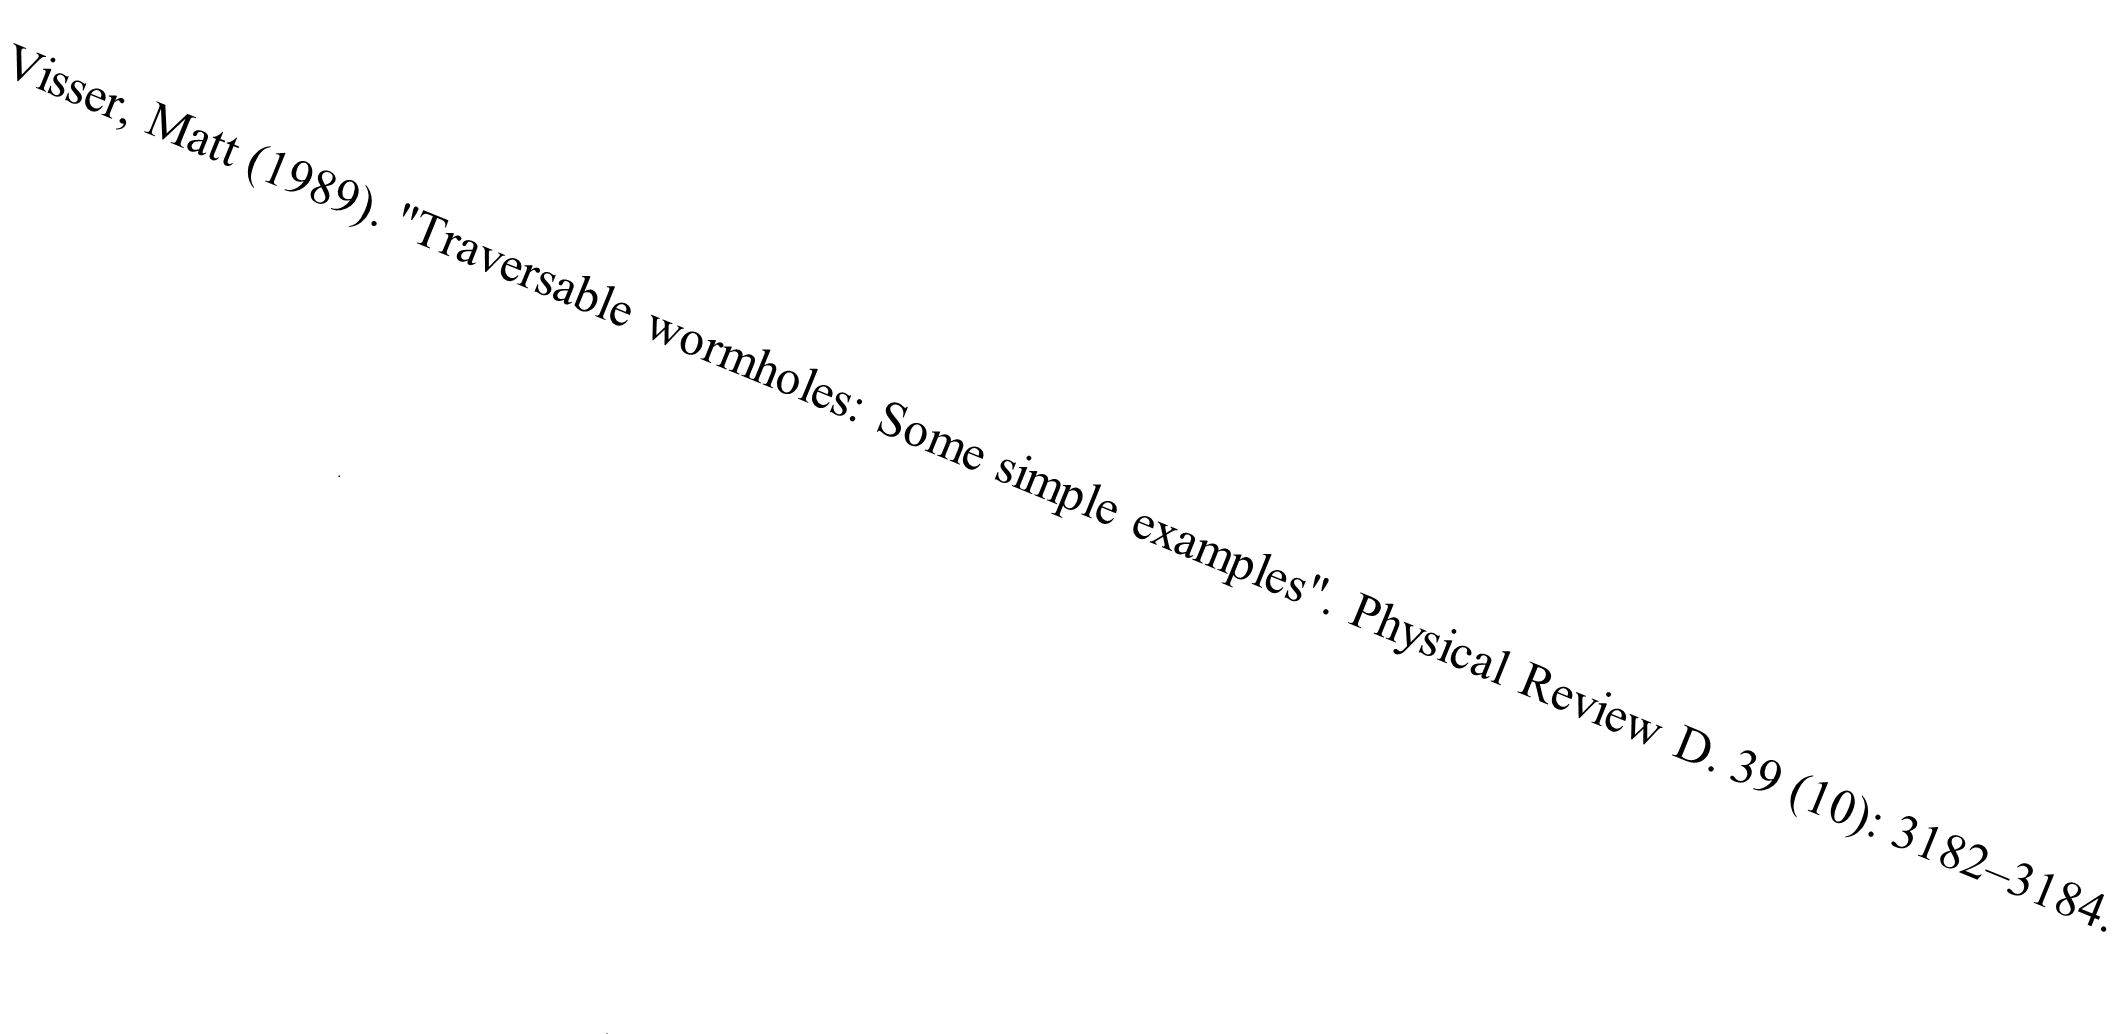
\includegraphics[scale=0.5]{../figures/oblique_reference.png}
\end{figure}

\section{preliminary results}
{\color{red} AMP: This temporary section is a summary of preliminary results that can help provide context and guide our thinking as we construct the story.  Specific results may or may not make it into the paper.}

The models referenced are:
\begin{itemize}
	\item wormholes -- This is a plan-view, DISV model that emulates a cross-sectional model and includes ``connector" cells that can have sloped tops and bottoms. Cell dimensions and hydraulic conductivities can be adjusted to approach a ``dip-following" mesh (in which cell tops and bottoms follow the dip of the channel) at one extreme and a vertically offset mesh (the kind MODFLOW actually uses in cross-section) at another extreme. A vertically offset mesh is approached by making the width of the connector cells very small in the x direction and, in the case of xt3d, making them anisotropic with very high K (1000 x the base K in these runs) along the slope of the cell and very low K (0.001 x the base K) perpendicular to the slope. The case of a vertically offset mesh using the standard formulation, which cannot implement such anisotropy, was run but is not generally of interest. This model is in the repo, but results from this model probably won't be included in the paper.
	\item crossconnected -- This is a plan-view, DISV model that emulates a cross-sectional model with ``cross-connections" between model layers. This model is not in the repo, and results are noted here primarily to confirm the expected agreement with the disu\_approach model.
	\item disu\_approach -- This implements cross-connections ``for real" in a cross-sectional, DISU model. Specific discharge is recalculated in the notebook to account for overlap areas; the recent ``patch" to MF6 is not being used (yet).
	\item transect\_benchmark -- This is the vertically offset model of \cite{bardot2022} updated to allow cross-connections. Results from this model are not summarized here yet.
\end{itemize}

In the model of \cite{bardot2022} and its transect\_benchmark update, the channel is embedded in a surrounding ``domain."  In each of the other three models, there is no surrounding domain -- the channel is the entire model. The distinction may be significant because the surrounding matrix provides vertical connections to the channel. When the surrounding domain is (effectively) impermeable, these vertical connections contribute ``zero vertical flux" information to the specific discharge calculation, implying that the specific discharge is literally horizontal. In the absence of a surrounding domain, there is no vertical flux component information. Need to check what difference this might make.

In the plan-view models, rows function as ``layers." Unless stated otherwise, all results are for a 30-degree channel dip, and the analytical solution is a specific discharge of 1. inclined at 30 degrees. Total flow is the sum of the flows reported for the CHD cells along the left end of the channel. Numerical results are rounded arbitrarily. The terms ``specific discharge" and ``flux" are using interchangeably.

\subsection{Single-layer channel}
The channel is represented using a single layer of cells.

\subsubsection{wormholes, 1x11 cells:}
Results were the same whether the mesh was vertically offset (xt3d and standard, though not sure if standard results are meaningful) or dip-following (xt3d and standard), which is not surprising since there are no connections across the tops and bottoms. The errors in computed heads were miniscule in all cases.

\paragraph{with xt3d:} Specific discharge is 0.8660 and ``seemingly" horizontal. This makes sense if you consider that the only connections in the model are ``horizontal" ones along the layer. A horizontal flux component of 0.8660 corresponds (via the cosine factor) to a unit flux from left to right along the dip of the channel, so in that sense it's correct. Furthermore, that's the only flux component that exists in this model, and therefore the only one xt3d can calculate; the vertical flux component is reported as zero by default. So rather than say the flux is horizontal, perhaps it's fairer to say MODFLOW gets the horizontal component right and simply can't tell us what the vertical component is. Total flow is 0.8660, which is correct.

\paragraph{without xt3d (standard formulation)} Specific discharge is 1.1547 and, again, ``seemingly" horizontal. This increase in magnitude relative to xt3d makes sense because the standard formulation ignores both the angle of the connection relative to the vertical cell interface and the reduction in area for flow (area perpendicular to the long axis of the channel) when the channel dips. Therefore, the  magnitude differs by a factor of $1/{(cosine factor)}^2$. Total flow is 1.1547, which reflects the error in the flux.

\subsubsection{crossconnected, 1x11 cells:} Specific discharge results are essentially identical to those in the vertically offset wormholes model, which is not surprising given that there can be no cross-connections in a single-layer model. The errors in computed heads were miniscule with and without xt3d.

\paragraph{with xt3d:} Total flow is 0.3660, which reflects the smaller area available for flow between two cells (the overlap area).

\paragraph{without xt3d (standard formulation)} Total flow is 0.4880, which (given the incorrect flux) also reflects the smaller area available for flow between two cells (the overlap area).

\subsubsection{disu\_approach, 1x11 cells:} Specific discharge results are essentially identical to those in the vertically offset wormholes model and crossconnected model. Total flow matched either the vertically offset wormholes result or the crossconnected result depending on how the ``staggered" flag was set in the notebook, which determined whether the specific discharge remained based on average areas or was recalculated using overlap areas. (There are no cross-connections in a single-layer model, so the cell-cell flows were unaffected, so it was just a matter of whether the fluxes were postprocessed to adjust the areas.) The errors in computed heads were miniscule with and without xt3d.

\subsection{Two-layer channel}
The channel is represented using two layers of cells. This introduces the possibility of vertical flows between layers.

\subsubsection{wormholes, 2x11 cells}

\paragraph{dip-following mesh with xt3d:} In the connector cells (which are of primary interest in this case), specific discharge is 0.9998 mid-channel and 1.00003 on average, with a max error of +0.0003. Angle of specific discharge is 29.9913 deg mid-channel and 29.9879 on average, with a max error of +0.03 deg. Errors in computed heads (including all cells) are on the order of 0.002\%. Total flow is 1.7321 (0.8661 per cell). So, good agreement with the analytical solution.

\paragraph{dip-following mesh without xt3d (standard formulation)} In the connector cells (which are of primary interest in this case), specific discharge is 1.3336 mid-channel and 1.3687 on average, with a max error of +0.69. Angle of specific discharge is 30.05 deg mid-channel and 32.24 on average, with a max error of +9.8 deg. Errors in computed heads (including all cells) are on the order of 2\%. Total flow is 2.3094 (1.1547 per cell).

\paragraph{vertically offset mesh with xt3d:} In the flat-top cells (which are of primary interest in this case), specific discharge is 1.1117 mid-channel and 1.1211 on average, with a max error of +0.35. Angle of specific discharge is -0.53 deg mid-channel and 6.0095 on average, with a max error of -30.54 deg; the flow generally skews toward horizontal. Errors in computed heads (including all cells) are on the order of 4\%. Total flow is 2.1993 (1.0997 per cell).

\subsubsection{crossconnected, 2x11 cells:}

\paragraph{with xt3d:} Specific discharge matches the analytical solution very closely, with a max error of -5e-9. Angle of specific discharge also matches very closely, with a max error of -9e-8 deg. Errors in computed heads are minscule. Total flow is 1.2321 (0.6161 per cell), which reflects the reduced area for flow; the non-overlapping area of the lowest left-hand boundary cell is effectively ``lost." Otherwise, a great result.

\paragraph{without xt3d (standard formulation)}  Specific discharge is 1.0922 mid-channel and 1.1074 on average, with a max error of +0.30. Angle of specific discharge is 22.69 deg mid-channel and 23.28 on average, with a max error of -7.5 deg. Errors in computed heads are on the order of 0.5\%. Total flow is 1.3942 (0.6971 per cell). Overall, not a great result, but not terrible; the cross-connections alone seem to have helped substantially.

\subsubsection{disu\_approach, 2x11 cells:}

\paragraph{without cross-connections, with xt3d:} Results are comparable to those in the wormhole model with a vertically offset mesh and xt3d. Specific discharge is 1.1045 mid-channel and 1.1262 on average, with a max error of +0.38. Angle of specific discharge is 0.0731 deg mid-channel and 6.2516 on average, with a max error of -29.93 deg; the flow generally skews toward horizontal. Errors in computed heads are on the order of 3\%. Total flow is 2.2091 (1.1045 per cell).

\paragraph{without cross-connections, without xt3d (standard formulation):} Specific discharge is 1.1547 mid-channel and 1.1755 on average, with a max error of +0.43. Angle of specific discharge is 0.0685 deg mid-channel and 5.9963 on average, with a max error of -29.93 deg; the flow generally skews toward horizontal. Errors in computed heads (including all cells) are on the order of 2\%. Total flow is 2.3094 (1.1547 per cell). Overall, comparable to the results with xt3d.

\paragraph{with cross-connections, with xt3d:} Results are comparable to those in the crossconnected model with xt3d. Specific discharge matches the analytical solution very closely, with a max error of +1e-8. Angle of specific discharge also matches very closely, with a max error of -3e-7 deg. Errors in computed heads are minscule. Total flow is 1.2321 (0.6161 per cell), which reflects the reduced area for flow; the non-overlapping area of the lowest left-hand boundary cell is effectively ``lost." Otherwise, a great result.

\paragraph{with cross-connections, without xt3d (standard formulation):} Results are comparable to those in the crossconnected model without xt3d. Specific discharge is 1.0948 mid-channel and 1.1101 on average, with a max error of +0.30. Angle of specific discharge is 22.63 deg mid-channel and 23.22 on average, with a max error of -7.5 deg. Errors in computed heads are on the order of 0.5\%. Total flow is 1.3942 (0.6971 per cell). Overall, not a great result, but not terrible; the cross-connections alone seem to have helped substantially.

\subsection{Five-layer channel}
The channel is represented using five layers of cells.

\subsubsection{wormholes, 5x11 cells:}

\paragraph{dip-following mesh with xt3d:} Results are basically similar to those in the 2-layer case, except the total flow is greater in proportion to the greater number of boundary cells.

\paragraph{dip-following mesh without xt3d (standard formulation)} Results are roughly comparable to but a bit worse overall than those in the 2-layer case. In the connector cells (which are of primary interest in this case), specific discharge is 1.3579 mid-channel and 1.4277 on average, with a max error of +1.14. Angle of specific discharge is 31.7497 deg mid-channel and 35.6924 on average, with a max error of +19.57 deg. Errors in computed heads (including all cells) are on the order of 8\%. Total flow is 5.7735 (1.1547 per cell). 

\paragraph{vertically offset mesh with xt3d:} Results are roughly comparable to those in the 2-layer case. In the flat-top cells (which are of primary interest in this case), specific discharge is 0.8906 mid-channel and 1.0013 on average, with a max error of +0.54. Angle of specific discharge is 2.8558 deg mid-channel and 10.9171 on average, with a max error of -31.5 deg; the flow generally skews toward horizontal. Errors in computed heads (including all cells) are on the order of 10\%. Total flow is 4.8426 (0.9685 per cell).

\subsubsection{crossconnected, 5x11 cells:}

\paragraph{with xt3d:} Results are basically similar to those in the 2-layer case. Total flow is 3.8301 (0.7660 per cell), which is better than the 2-layer result due to the ``lost" (non-overlapping) area being a smaller proportion of the total area for flow.

\paragraph{without xt3d (standard formulation)}  Results are basically comparable to those in the 2-layer case, except the errors in computed heads are substantially higher at around 1.5\%, and the total flow of 4.0944 gives a somewhat higher flow per cell at 0.8189. Again, not great, but not terrible.

\subsubsection{disu\_approach, 5x11 cells:}

\paragraph{without cross-connections, with xt3d:} Results are roughly comparable to but a bit worse overall than those in the 2-layer case. Specific discharge is 1.0547 mid-channel and 1.0926 on average, with a max error of +0.62. Angle of specific discharge is 2.9627 deg mid-channel and 10.3771 on average, with a max error of -28.1 deg; the flow generally skews toward horizontal. Errors in computed heads are on the order of 8\%. Total flow is 5.3106 (1.0621 per cell).

\paragraph{without cross-connections, without xt3d (standard formulation):} Results are roughly comparable to but a bit worse overall than those in the 2-layer case. Specific discharge is 1.1560 mid-channel and 1.1827 on average, with a max error of +0.70. Angle of specific discharge is 2.7571 deg mid-channel and 9.5527 on average, with a max error of -28.3 deg; the flow generally skews toward horizontal. Errors in computed heads (including all cells) are on the order of 8\%. Total flow is 5.7735 (1.1547 per cell). Overall, comparable to the results with xt3d.

\paragraph{with cross-connections, with xt3d:} Results are basically similar to those in the 2-layer case. Total flow is 3.8301 (0.7660 per cell), which is better than the 2-layer result due to the ``lost" (non-overlapping) area being a smaller proportion of the total area for flow.

\paragraph{with cross-connections, without xt3d (standard formulation):} Results are comparable to those in the crossconnected model without xt3d. Again, not great, but not terrible.

\subsection{Crossflow}
What happens if the flow is across the channel rather than along it? Using cross-connections together with xt3d appears to help when only the channel is simulated (no domain). With the domain present, the results are thrown off considerably by the lack of a ``heterogeneity correction" in the xt3d interpolation, though the errors may be concentrated near the channel boundary.  Will not get too much into the crossflow case in this paper, but could mention the heterogeneity correction as ongoing work.

\begin{figure}[H]
\centering
\begin{subfigure}{0.4\textwidth}
	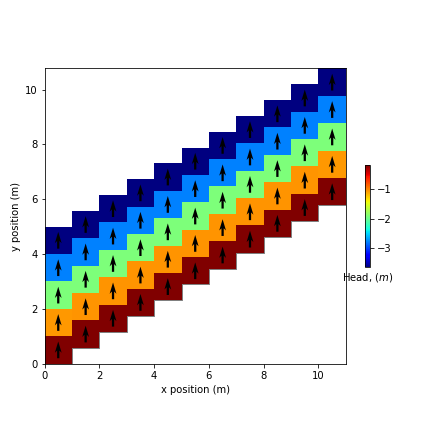
\includegraphics[width=\textwidth]{../figures/disu-cf-vo-s-head.png}
	\caption{standard conductance-based formulation}
	\label{fig:disu-s-nocc-cf-head.}
\end{subfigure}
\hfill
\begin{subfigure}{0.4\textwidth}
	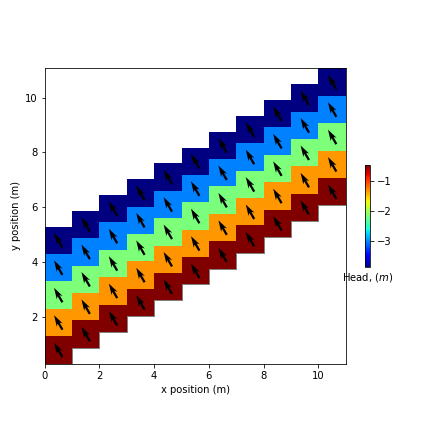
\includegraphics[width=\textwidth]{../figures/disu-cf-vo-x-head.png}
	\caption{XT3D}
	\label{fig:disu-x-nocc-cf-head}
\end{subfigure}
\caption{Specific discharge and head for a vertically offset grid and boundary heads set up for crossflow. The standard formulation is a fail, but XT3D nails it, even without cross-connections. (preliminary result from disu\_approach model, 5x11 grid without cross-connections, $30^{\circ}$ incline, set up for flow across the channel; scenarios disu-cf-vo-s and disu-cf-vo-x)}
\label{fig:figures}
\end{figure}

\begin{figure}[H]
\centering
\begin{subfigure}{0.4\textwidth}
	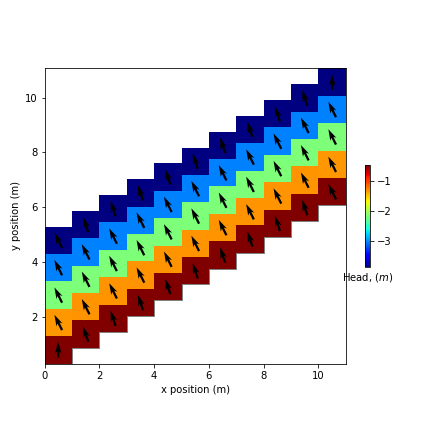
\includegraphics[width=\textwidth]{../figures/disu-cf-vs-s-head.png}
	\caption{standard conductance-based formulation}
	\label{fig:disu-s-cc-cf-head}
\end{subfigure}
\hfill
\begin{subfigure}{0.4\textwidth}
	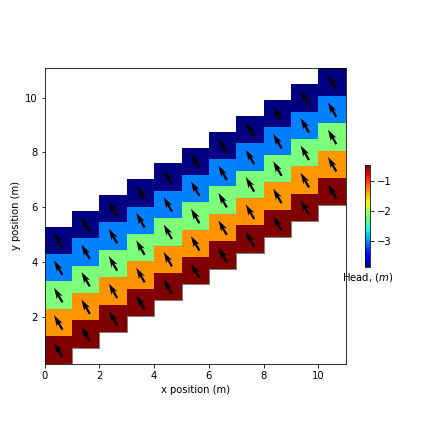
\includegraphics[width=\textwidth]{../figures/disu-cf-vs-x-head.png}
	\caption{XT3D}
	\label{fig:disu-x-cc-cf-head}
\end{subfigure}
\caption{Specific discharge and head for a vertically staggered grid with cross-connections and boundary heads set up for crossflow. The standard formulation does pretty well, and XT3D nails it. (preliminary result from disu\_approach model, 5x11 grid with cross-connections, $30^{\circ}$ incline, set up for flow across the channel; scenarios disu-cf-vs-s and disu-cf-vs-x)}
\label{fig:figures}
\end{figure}

\begin{figure}[H]
\centering
\begin{subfigure}{0.4\textwidth}
	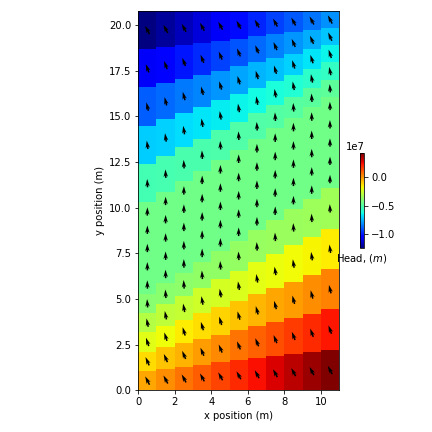
\includegraphics[width=\textwidth]{../figures/disu-d-cf-vo-s-head.png}
	\caption{standard conductance-based formulation}
	\label{fig:disu-s-nocc-cf-head.}
\end{subfigure}
\hfill
\begin{subfigure}{0.4\textwidth}
	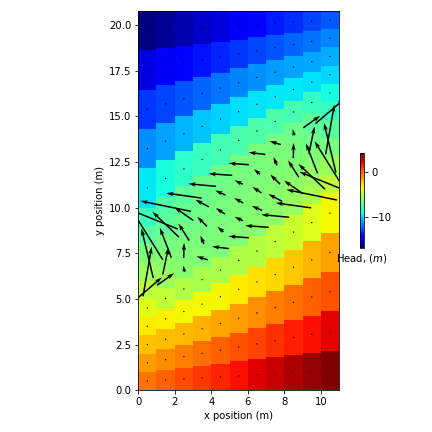
\includegraphics[width=\textwidth]{../figures/disu-d-cf-vo-x-head.png}
	\caption{XT3D}
	\label{fig:disu-x-nocc-cf-head}
\end{subfigure}
\caption{Specific discharge and head for a vertically offset grid with the domain and boundary heads set up for crossflow. The standard formulation gives nearly vertical flow in the channel, and XT3D also does poorly, even mid-channel. The huge specific discharge vectors near the channel boundary are apparently caused by XT3D's head-gradient interpolation drawing heads from the domain, where the head gradient is huge, when computing nominally horizontal flows between cells within the channel. (preliminary result from disu\_approach model, 5x11 channel with 5x11 subdomains above and below, without cross-connections, $30^{\circ}$ incline, set up for flow across the channel; scenarios disu-d-cf-vo-s and disu-d-cf-vo-x)}
\label{fig:figures}
\end{figure}

\begin{figure}[H]
\centering
\begin{subfigure}{0.4\textwidth}
	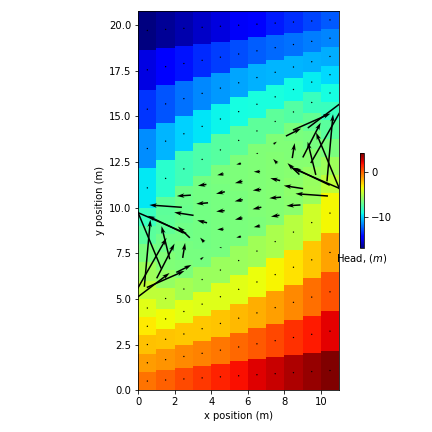
\includegraphics[width=\textwidth]{../figures/disu-d-cf-vs-s-head.png}
	\caption{standard conductance-based formulation}
	\label{fig:disu-s-cc-cf-head}
\end{subfigure}
\hfill
\begin{subfigure}{0.4\textwidth}
	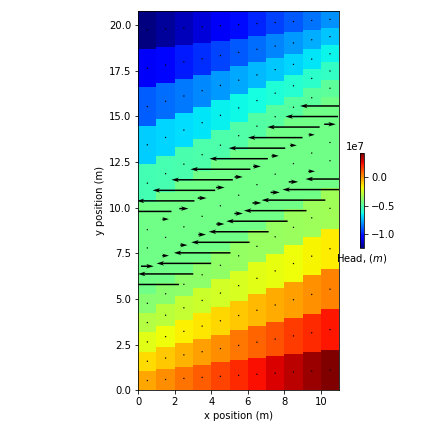
\includegraphics[width=\textwidth]{../figures/disu-d-cf-vs-x-head.png}
	\caption{XT3D}
	\label{fig:disu-x-cc-cf-head}
\end{subfigure}
\caption{Specific discharge and head for a vertically staggered grid with the domain and with cross-connections and boundary heads set up for crossflow. The standard formulation is much improved. You can't tell because of the scale of the vectors, but XT3D does well mid-channel. However, near the channel boundary it still has huge flows due to interpolating heads from the domain. (preliminary result from disu\_approach model, 5x11 channel with 5x11 subdomains above and below, $30^{\circ}$ incline, set up for flow across the channel; scenarios disu-d-cf-vs-s and disu-d-cf-vs-x)}
\label{fig:figures}
\end{figure}

\subsection{Domain}
Results with the surrounding "domain" (from an updated disu\_approach notebook) are similar but not identical, apparently due to the "staircase" effect. Original thought was to present most of our results without the domain, at least when illustrating the main problem and its solution (to keep the "theory" clear), then discuss what happens when the domain is present (which is more like in practice). Kerry has suggested the results with the domain are sufficient.

\end{document}
